\documentclass{article}

\usepackage[normalem]{ulem}
\usepackage{fancyhdr}
\usepackage[parfill]{parskip}
\usepackage{tikz}
\pagestyle{fancyplain}

\title{Negative feedback}
\author{Todd Davies}
\date{\today}

\begin{document}

\rhead{Negative feedback}
\lhead{\today}

\maketitle

\section*{Negative feedback}
\thispagestyle{empty}

Negative feedback is a mechanism that restores systems to their original level.
It does this by doing the opposite of any change to the system. For example, if
the body temperature becomes too high, then the body will start to sweat until
the temperature has dropped again.

Different methods of controlling a single system can effect it in multiple ways.
Continuing the body temperature example, if the body becomes too cold, then the
rate of respiration will be increased and the person will begin to shiver to
increase the temperature.

This shows how multiple factors can change a system in multiple ways to provide
a great degree of control, and multiple factors can also change a system in the
same way to give redundancy and increased effectiveness.

\section*{Positive feedback}

Positive feedback is essentially the opposite of negative feedback. It results
in greater departures from a system's original level. Positive feedback is often
used to respond quickly to a stimuli, for example to stimulate the formation of
a blood clot after an injury.

Positive feedback can also happen when the homeostatic system breaks down and
fails. If you are too cold for too long, your body temperature may drop
drastically very quickly.

\section*{The menstrual cycle}

The meustrual cycle lasts around 28 days. It involves the following stages:

\begin{enumerate}

	\item An egg cell starts to ripen inside a follicle.

	\item Ovulation occurs as an egg is released.

	\item The uterus lining becomes thicker to the egg can implant.

	\item The corpus luteum developes around the egg in the uterus wall.

	\item If there is no fertilisation the thick wall of the uterus breaks down
	and exits the body through the vagina (menstruation).

\end{enumerate}

Menstruation is controlled by the action of four hormones shown in the table
below:

\begin{center}
	\begin{tabular}{|l|p{5cm}|l|}
		\hline

		{\bf Name} & {\bf Function} & {\bf Site of production}\\ \hline

		FSH & Stimulates the follicle to develop. & Pituitary gland\\ \hline

		LH & Stimulates ovulation and the development of the corpus luteum. &
		Pituitary gland\\ \hline

		Oestrogen & Stimulates the thickening of the uterus lining. & Ovaries\\ \hline

		Progesterone & Maintains the thick uterus lining, ready for implantation
		of an embryo. & Ovaries\\ \hline

	\end{tabular}
\end{center}

You don't need to learn this, but here's a graph of what is happening throughout
the month:

\begin{center}
	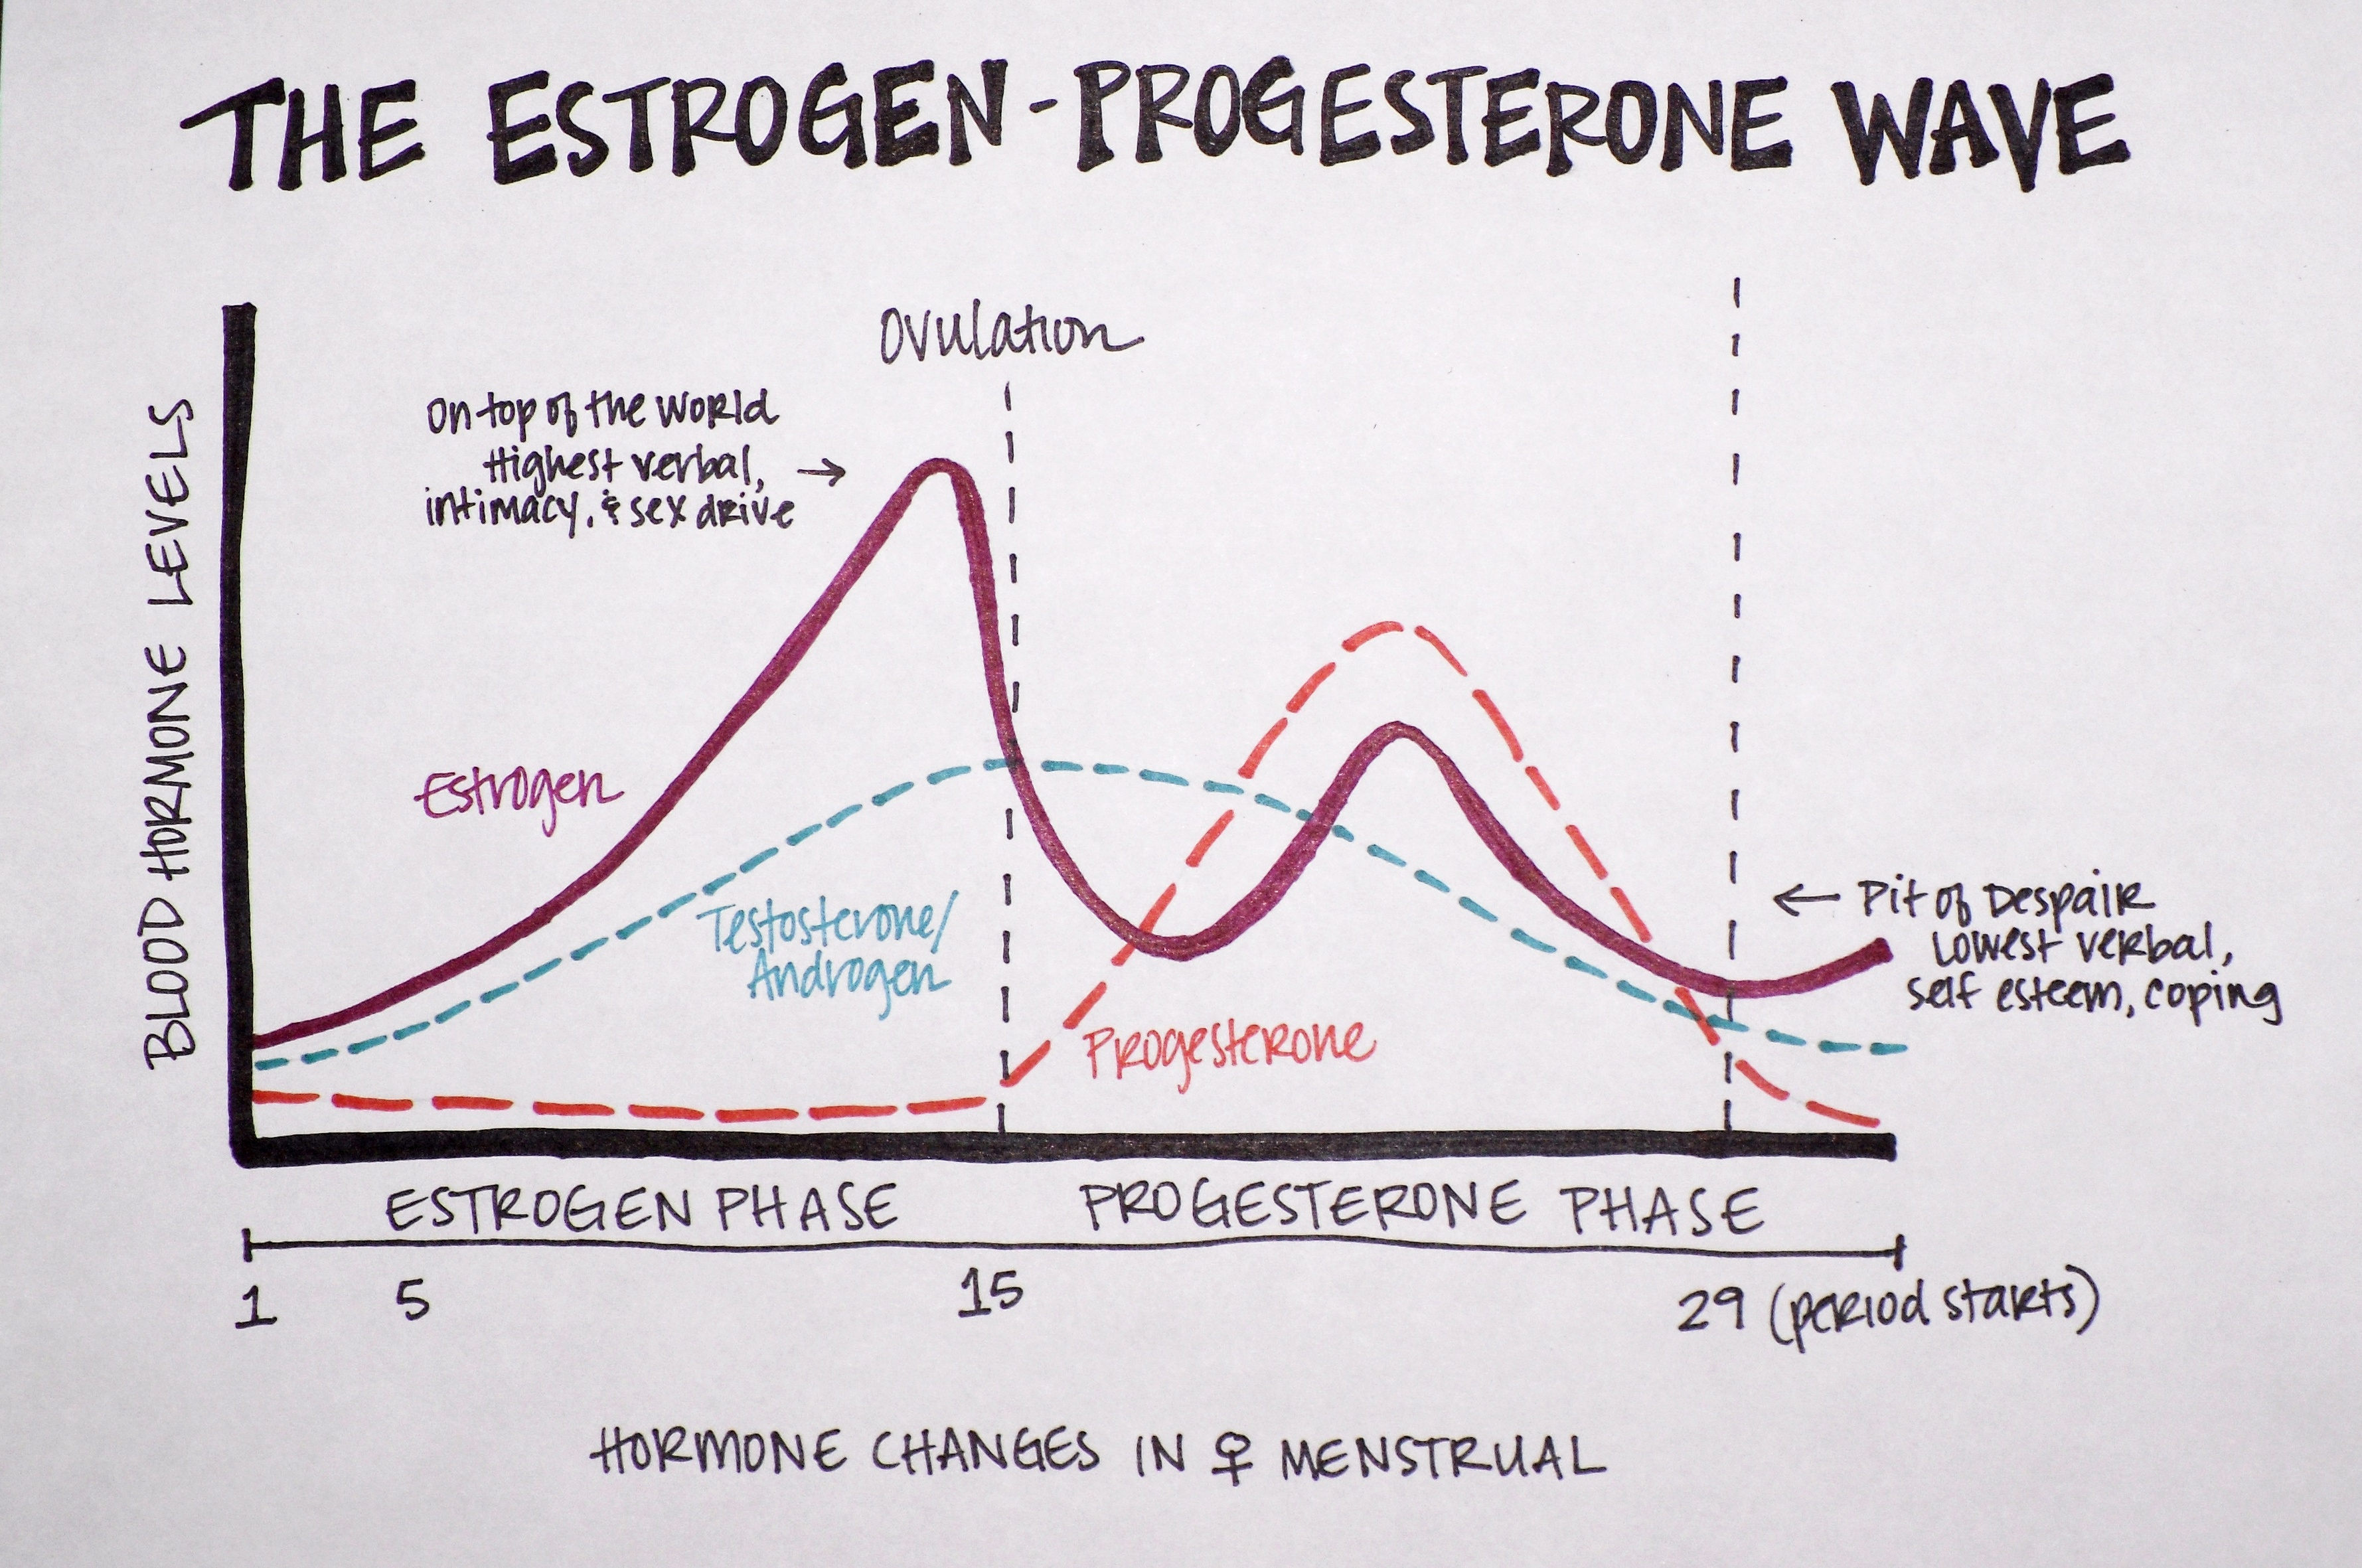
\includegraphics[angle=0,scale=0.15]{menstrual_cycle}
\end{center}

\end{document}